\chapter{Proof-of-Concept: Sprachnachrichten}
Neben der klassischen Chatbot-Funktion, bei der ein User per Textnachrichten mit dem Bot redet, ist es vor allem in letzter Zeit immer mehr zum Usus geworden, dass man mit Bots reden möchte, um Informationen zu erhalten.  \\Produkte wie Google Home und Amazons Alexa sind hierfür die bekanntesten Vertreter, die eine solche Funktion bieten. Während des Brainstormings zu Use-Cases des Chatbots kam zudem die Idee auf, dass der Chatbot nicht nur auf Chat-Nachrichten antworten, sondern auch auf Sprachnachrichten reagieren können sollte. \\
Hier bietet Telegram die Möglichkeit, kurze Sprachnachrichten direkt zu versenden. Wenn der Bot diese Sprachnachricht zu Text übersetzen könnte, ist es möglich, diesen verstandenen Text durch den Chatbot zu verarbeiten und entsprechend zu antworten. \\
Da der produktive Einsatz eines solchen Features nicht wahrscheinlich ist, sollte es als Proof-of-Concept untersucht und exemplarisch implementiert werden.

\section{Architekturentwurf}
Telegram bietet mit seinen Sprachnachrichten bereits die Möglichkeit, Sprache aufzunehmen und zu versenden. Diese Sprachnachrichten können nicht nur zwischen zwei Personen verschickt werden, sondern auch zwischen einer Person und einem Bot versandt werden. Telegram unterstützt die mobilen Betriebssysteme \texttt{iOS} und \texttt{Android}. Am Desktop lässt es sich über \texttt{MacOS}, \texttt{Windows}, \texttt{Linux} und im Webbrowser bedienen. Durch eine direkte Integration in diese Telegram-Clients, ist es also sehr einfach, solche Nachrichten zu versenden.

\subsection{Speech-to-Text}
Die Interpretation der Sprachnachricht erfolgt durch Rivescript, was Texteingaben verarbeitet und Textausgaben erzeugt. Somit ist es notwendig, dass die Spracheingabe zu Text verarbeitet wird, was im Allgemeinen als Speech-to-Text bezeichnet wird. Diese Umwandlung ist nicht trivial und wird mittels Machine-Learning möglich gemacht. Anstatt die Umwandlung selber zu machen, wurde sie in diesem Projekt exemplarische Googles-Cloud-Services erzeugt. Google setzt auf Machine-Learning und hat durch seine große Nutzerzahl und vielseitige Nutzung gut trainierte Modelle, sodass die Sprache zuverlässig verstanden werden kann.

\subsection{Google-Cloud-Speech-API}
Die Google-Cloud-Speech-to-Text-API ist ein SAAS-Angebot, bei dem man Sprachdateien an den Google-Server senden kann und diese Sprachdateien von dem Service interpretiert und zu Text umgewandelt werden, den man als einfaches JSON-Objekt erhält. Da die Umwandlung von Sprache zu Text auf der Wahrscheinlichkeit beruht, dass etwas korrekt verstanden wurde, wird diese Genauigkeit mitzurückgegeben. Sollte die Eingabesprache nicht eindeutig sein, so werden mehrere Ergebnisse mit der jeweiligen Genauigkeit zurückgegeben.
Der Cloud-Service wird über HTTP angesprochen, man muss jedoch eine Authentifizierungstoken einreichen. Hierfür muss man sich einen Google-Developer-Account erstellen und muss die API aktivieren. Der Service kostet für gewöhnlich Geld, hierbei werden 0,006\$/15 Sekunden berechnet.\footnote{\url{https://cloud.google.com/speech-to-text/}} \\
Man kann den Service jedoch kostenlos nutzen, wenn man pro Tag weniger als 60 Minuten an Eingabe verarbeitet. Zusätzlich erhält man bei der Eröffnung eines Accounts ein Guthaben in Höhe von 300\$, sodass man die Services ausgiebig testen kann.

Das folgende Schaubild soll einen exemplarischen Ablauf erklären:
\begin{figure}[H]
    \centering
    \caption{Kommunikationsprozess}
      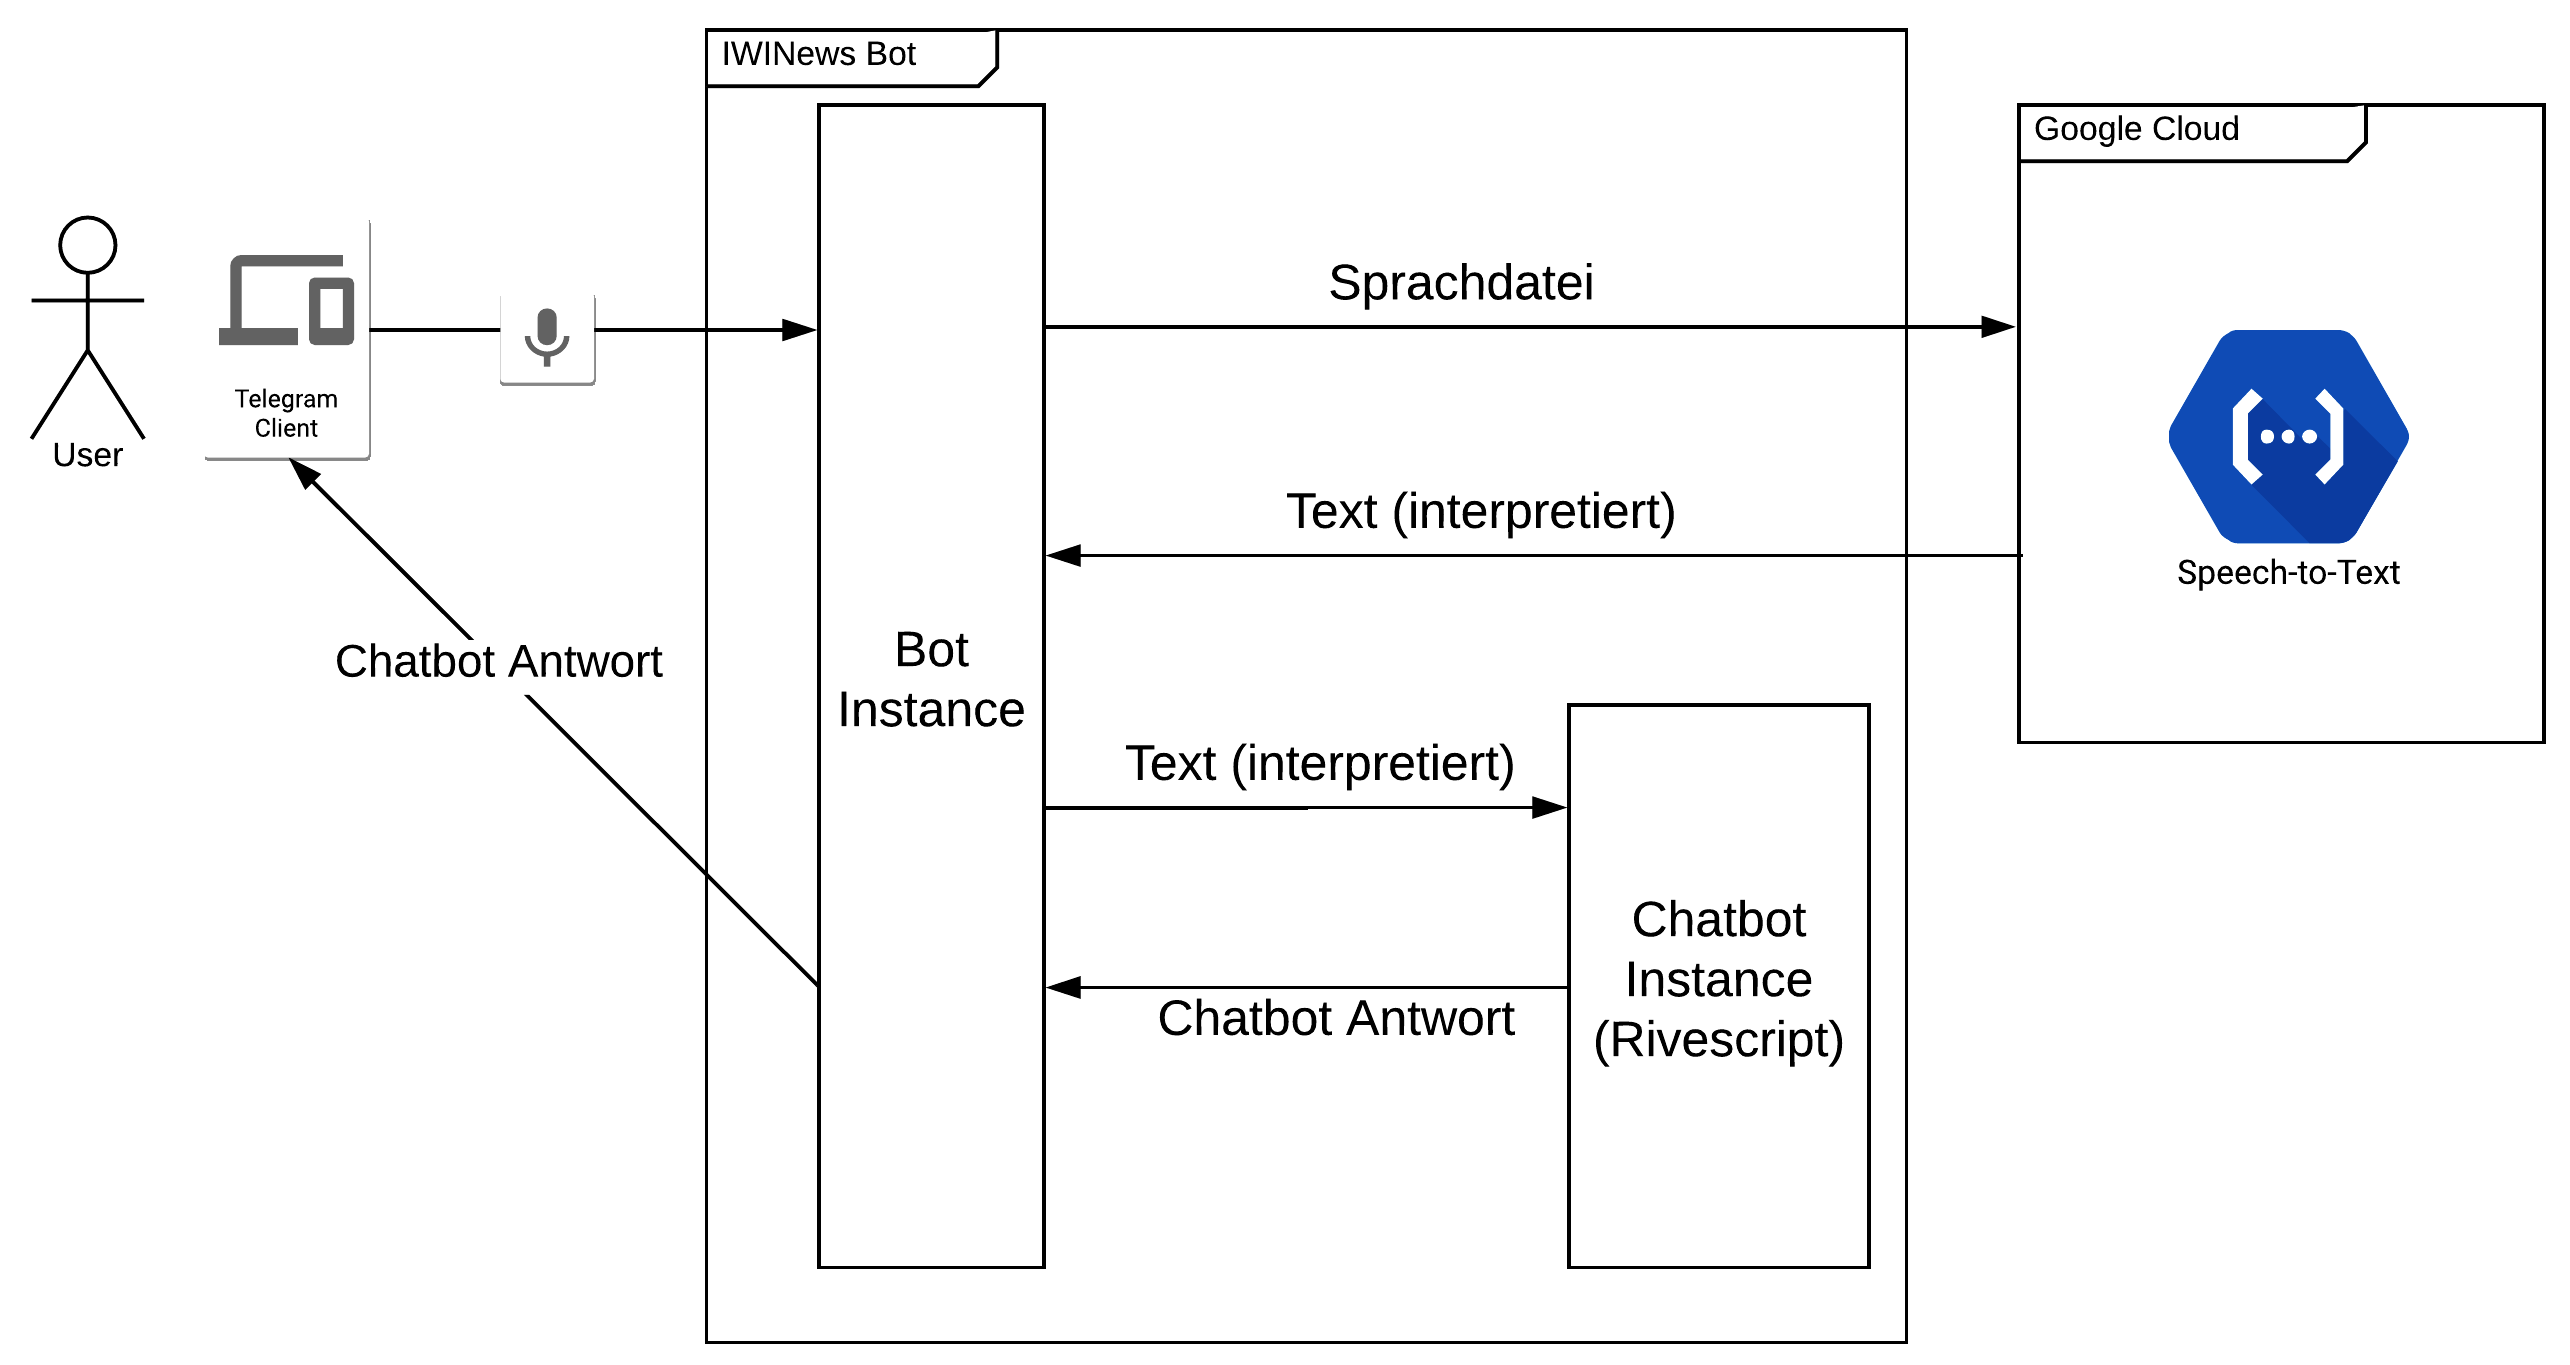
\includegraphics[width=\linewidth]{ArchitekturTelegramBot.png}
      \label{img:architektur}
    \caption*{Quelle: Eigene Abbildung}
\end{figure}

\subsubsection{Java-Bibliothek}
Google bietet eine Java-Bibliothek an, um den Aufruf der API zu abstrahieren und somit zu vereinfachen. Hierbei wird sowohl die Authentifizierung, als auch die Anfrage mit den einzelnen Parametern stark vereinfacht. Diese Bibliothek befindet sich jedoch noch im Alpha-Modus und sollte somit auf keinen Fall in produktiven Umgebungen eingesetzt werden. Auch in diesem Projekt sind Warnungen beim Bauen mit \texttt{sbt} aufgetreten und es wurde ein Issue auf Github eröffnet, sodass dieses Problem für das Release gefixt wird.\footnote{\url{https://github.com/GoogleCloudPlatform/google-cloud-java/issues/3329}} 
Die Einbindung der Bibliothek ist jedoch sehr einfach, da sie auf Maven-Central gehostet wird.

\subsubsection{Authentifizierung}
Das Token, das zur Authentifizierung genutzt wird, ist in einer \texttt{.json}-Datei gespeichert, die man in der Google-Developer-Console downloaden kann. Diese \texttt{.json}-Datei muss dem Programm, das die Google-API ansprechen möchte, bekannt gemacht werden, was am einfachsten über die Pfadvariable \texttt{GOOGLE\_APPLICATION\_CREDENTIALS} gemacht wird. Diese Pfadvariable wird dann von der Bibliothek gelesen und zur Authentifizierung genutzt. Da in der Pfadvariable nicht der Inhalt der \texttt{.json}-Datei, sondern der Pfad zur \texttt{.json}-Datei gespeichert wird, darf man diese Datei nicht löschen oder verschieben.

\section{Implementierung}
Nachdem nun die relevanten Technologien und deren Zusammenspiel beschrieben wurden, soll vorgestellt werden, wie die Interpretation der Sprachnachrichten konkret funktioniert und wie es umgesetzt wurde.

\subsubsection{Beispiel}
Bevor auf die Implementierungsdetails eingegangen wird, soll die Funktionsweise vorgestellt und erläutert werden.

\begin{figure}[!htb]
    \centering
    \caption{Beispiel der Verwendung von Speech-to-Text}
      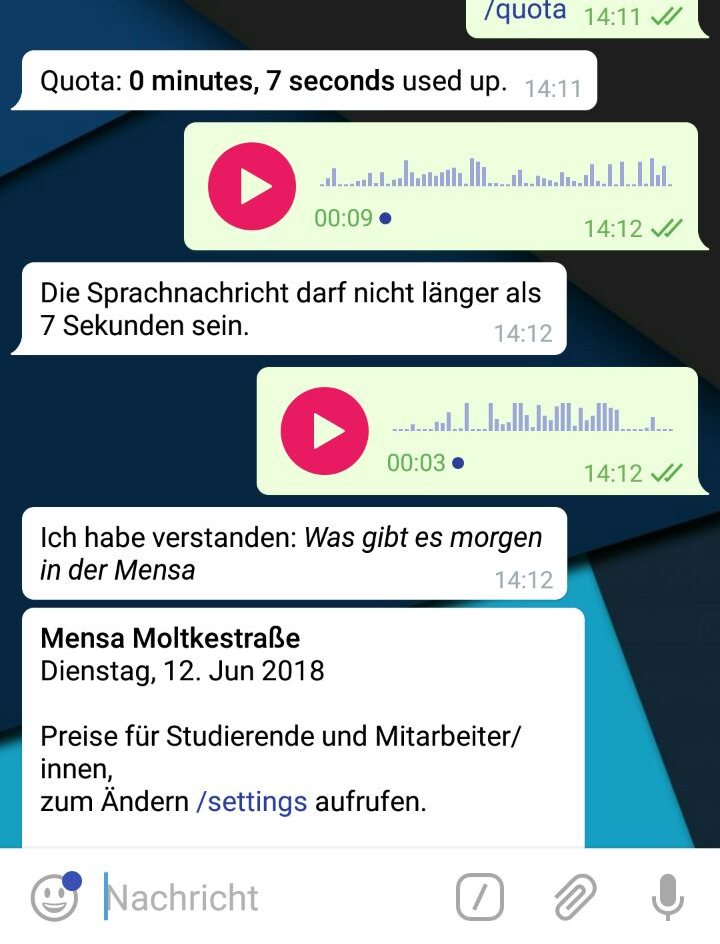
\includegraphics[width=0.5\linewidth]{Sprachnachrichten_Beispiel.png}
      \label{img:speekExample}
    \caption*{Quelle: Eigene Abbildung}
\end{figure}

Wie man an dem Beispiel bereits erkennt, gibt es eine Quota, die speichert, wie viel von dem Kontingent für Sprachnachrichten bereits verbraucht wurde. Außerdem werden zu lange Nachrichten, also Nachrichten die Länger als sieben Sekunden dauern, abgewiesen. Durch diese Mechanismen wird vermieden, dass die Sprachnachrichten missbraucht werden und die Ressourcen des Google-Cloud-Service zu sehr beansprucht werden.
Neben den Einschränkungen erkennt man aber an dem Beispiel zusätzlich, dass die Sprachnachricht von dem Bot korrekt erkannt wird und anschließend vom Chatbot beantwortet wird.

\subsection{Empfang von Sprachnachrichten}
So wie bereits für die Chat-Nachrichten, muss der Bot so erweitert werden, dass er Sprachnachrichten empfangen kann. Dies geschieht über das Reagieren auf eingehende Nachrichten und das Überprüfen, ob es sich um eine Sprachnachricht handelt. Ist dies der Fall, so können bereits Eigenschaften der Sprachnachricht abgefragt werden, beispielsweise die Dauer. Dies ist sinnvoll, da über die Dauer entschieden wird, ob die Nachricht verarbeitet wird, oder nicht.

\todo{add code}

Wie man an diesem Code bereits erkennt, wird die Quota in der Redis-Datenbank gespeichert, sodass diese persistiert wird. Der User wird in dem Fall, dass die Quota für den Tag überschritten wird, mit einer Fehlermeldung über den Umstand informiert, zusätzlich wird der Vorfall geloggt. \\
Sollte die Quota noch nicht erschöpft sein und die Sprachnachricht ist kurz genug, wird die Datei geladen. Telegram sieht hierbei vor, dass ein Link generiert werden muss, über den die Sprachdatei dann geladen werden kann. Der Link folgt der folgenden Struktur:

\url{https://api.telegram.org/file/botBottoken/Filetoken}

Das Bot-Token ist dabei das Token, das zu Identifizierung des Telegram-Bots genutzt wird und in der Datei \texttt{bot.token} gespeichert ist. Das File-Token muss erst generiert werden. Für die Generierung dieses File-Tokens bietet das \texttt{Telegrambot4s}-Framework einen eigenen \texttt{request}-Aufruf an, der dieses Token als \texttt{filePath} zurückgibt. Dies geschieht wie folgt:

\todo{add code}

Über die URL kann dann die Sprachdatei heruntergeladen werden. Diese wird lokal in dem Ordner \texttt{voices/} abgelegt, dabei wird das Datum und die Uhrzeit, sowie die \texttt{userID} im Dateinamen gespeichert.
Diese Datei wird benötigt, um die darin enthaltene Sprache in Text umzuwandeln. Hier kommt also der Google-Cloud-Service ins Spiel.

\subsection{Konfiguration des Speech-Client}
Die Google-Cloud-API bietet eine Klasse des Typs \texttt{SpeechClient} an, über die die einzelnen Anfragen an den Google-Cloud-Service gestellt werden. Dieser muss entsprechend konfiguriert sein, damit die in den Sprachdateien enthaltene Sprache auch korrekt verstanden und zu Text transkribiert werden kann. \\
Die Sprachdateien liegen im \texttt{OGG}-Dateiformat vor. Ein Großes Problem bei der Entwicklung war dabei die Frequenz, da diese dem SpeechClient mitgeteilt werden muss. Hier wurde davon ausgegangen, dass alle Telegram-Clients auf das selbe Dateiformat mit derselben Frequenz setzen, was aber nicht der Fall ist. Gibt man die falsche Frequenz einer Sprachdatei an, kann Google den Inhalt nicht verstehen und gibt ein leeres Ergebnis zurück. Der Fehler fiel beim Testen mit verschiedenen Geräten auf und die Behebung erfolgte durch reines Herumprobieren bei den Frequenzen. \\
Nachdem das Problem lokalisiert wurde, war die Lösung verhältnismäßig einfach. Die Frequenz der lokalen Datei wird aus der Datei gelesen und dem SpeechClient mitgeteilt. Hierzu wird eine zusätzliche Bibliothek benötigt, die diese Funktion bereitstellt. Außerdem muss dem SpeechClient mitgeteilt werden, um welche Sprache es sich bei der Eingabe handelt, diese Erkennung erfolgt nicht automatisch. Die vollständige Konfiguration wird im Folgenden gezeigt.

\todo{add code}

Da die Bibliothek für Java-Programme geschrieben wurde, gilt es, das Ergebnis in eine Scala-Collection umzuwandeln, um die Ergebnisliste einfacher traversieren zu können.

Das erste Ergebnis ist für gewöhnlich das beste Ergebnis, dies wird an die Rivescript-Instanz übergeben und dort weiter verarbeitet. Dies geschieht wie bereits mit den Textnachrichten. \\
Kann eine Sprachnachricht nicht verstanden werden, etwa weil die Umgebungsgeräusche zu laut sind oder der Sprecher zu undeutlich spricht, wird entsprechend eine Fehlermeldung ausgegeben. \\
Bei jeder Anfrage an den Google-Cloud-Service wird die Dauer der Sprachnachricht der Quota hinzugefügt.
